% Short plain-language talk for the advisor: the paper bottom-up, one idea per frame.
% Same theme as talk.tex. Build: pdflatex prof_talk.tex (twice). Figures: figs/.
% Speaker notes are \note{} blocks. To print them, add \setbeameroption{show notes on second screen=right}.
\documentclass[aspectratio=169,11pt]{beamer}

\newcommand{\talkauthor}{Arnav Kapoor}
\newcommand{\talkinstitute}{IISER Bhopal}

\usepackage[T1]{fontenc}
\usepackage{lmodern}
\usepackage{booktabs,colortbl,xcolor,amsmath,amssymb}
\usepackage{tikz}
\usetikzlibrary{positioning,arrows.meta,calc}

\definecolor{ibar}{HTML}{0B3C6E}
\definecolor{iaccent}{HTML}{2A78D6}
\definecolor{iorange}{HTML}{EB6834}
\definecolor{igreen}{HTML}{0F8A5F}
\definecolor{ifoot}{HTML}{E9EEF4}
\definecolor{ink}{HTML}{1F1F1E}
\definecolor{muted}{HTML}{6B6A63}

\usefonttheme{professionalfonts}
\setbeamertemplate{navigation symbols}{}
\setbeamercolor{normal text}{fg=ink,bg=white}
\setbeamercolor{structure}{fg=ibar}
\setbeamercolor{frametitle}{fg=white,bg=ibar}
\setbeamerfont{frametitle}{size=\large,series=\bfseries}
\setbeamertemplate{itemize item}{\color{iaccent}\raisebox{0.15ex}{\scriptsize$\blacksquare$}}
\setbeamertemplate{frametitle}{%
  \nointerlineskip
  \begin{beamercolorbox}[wd=\paperwidth,ht=2.6ex,dp=1.3ex,leftskip=1.2em,rightskip=1.2em]{frametitle}
    \usebeamerfont{frametitle}\insertframetitle
  \end{beamercolorbox}
  \vspace{-0.2ex}{\color{iaccent}\rule{\paperwidth}{1.2pt}}\vspace{0.4ex}}
\setbeamertemplate{footline}{%
  \leavevmode\hbox{\scriptsize%
  \begin{beamercolorbox}[wd=.30\paperwidth,ht=2.4ex,dp=1ex,leftskip=1em]{author in head/foot}%
    \color{white}\talkauthor\end{beamercolorbox}%
  \begin{beamercolorbox}[wd=.48\paperwidth,ht=2.4ex,dp=1ex,center]{title in head/foot}%
    \color{ink}\insertshorttitle\end{beamercolorbox}%
  \begin{beamercolorbox}[wd=.22\paperwidth,ht=2.4ex,dp=1ex,right,rightskip=1em]{date in head/foot}%
    \color{ink}\insertframenumber/\inserttotalframenumber\end{beamercolorbox}}}
\setbeamercolor{author in head/foot}{bg=ibar}
\setbeamercolor{title in head/foot}{bg=ifoot}
\setbeamercolor{date in head/foot}{bg=ifoot}

\newcommand{\ours}[1]{\textcolor{iaccent}{\textbf{#1}}}
\newcommand{\orig}[1]{\textcolor{iorange}{#1}}
\newcommand{\opt}[1]{\textcolor{igreen}{#1}}
\newcommand{\src}[1]{\par\vfill{\scriptsize\color{muted}#1}}
\newcommand{\takeaway}[1]{\par\vfill{\setlength{\fboxsep}{6pt}\colorbox{ifoot}{\parbox{\dimexpr\linewidth-12pt}{\color{ibar}\textbf{#1}}}}}
% a rounded box for diagrams
\tikzset{card/.style={draw=ibar!25,fill=ifoot,rounded corners=4pt,align=center,inner sep=6pt,font=\small},
         hot/.style={card,fill=iaccent,draw=iaccent,text=white},
         arr/.style={-{Stealth[length=7pt]},very thick,muted}}
\newcommand{\bignum}[3]{\begin{tikzpicture}\node[card,text width=#1,font=\normalsize]{{\Huge\bfseries\color{#2}#3}};\end{tikzpicture}}

\title[Making quantum circuits shorter]{Making quantum circuits shorter,\\and proving how short they can get}
\author{\talkauthor}

\begin{document}

% ================================================================ 1 title
{\setbeamertemplate{footline}{}
\begin{frame}[plain]
  \begin{tikzpicture}[remember picture,overlay]
    \fill[ibar] (current page.south west) rectangle (current page.north east);
    \node[anchor=north west,text=iorange!70!white,font=\small\bfseries] at ([xshift=2.4em,yshift=-2em]current page.north west) {PROGRESS UPDATE};
    \node[anchor=west,text=white,text width=0.85\paperwidth,align=left] at ([xshift=2.4em,yshift=1.2em]current page.west)
      {{\LARGE\bfseries Making quantum circuits shorter,\\[0.2em] and proving how short they can get}\\[1em]
       {\large\color{white!75!ibar} What the original paper does, what we added, and what the numbers say}};
    \node[anchor=south west,text=white!65!ibar,font=\small] at ([xshift=2.4em,yshift=2em]current page.south west)
      {\talkauthor\ \textperiodcentered\ \talkinstitute\ \textperiodcentered\ qcr extension paper \textperiodcentered\ October 2026};
  \end{tikzpicture}
\end{frame}}
\note{Goal: walk from the basics up to our results, one idea per slide. The story in one line: the original method is far
from optimal, we can prove that, and a better general optimiser closes the gap and also works on real algorithm circuits.}

% ================================================================ 2 basics
\begin{frame}{Every gate costs reliability}
\begin{columns}[c]
\begin{column}{0.56\textwidth}
\centering
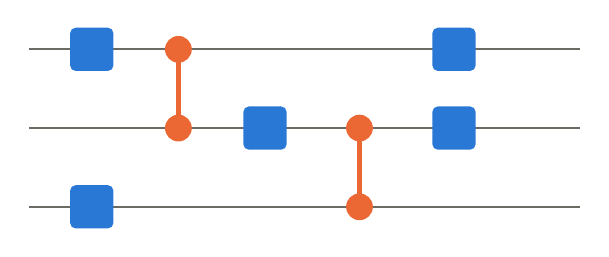
\begin{tikzpicture}[x=1cm,y=1cm]
  \foreach \y in {0,1,2} \draw[thick,muted] (0,\y) -- (7,\y);
  \foreach \x/\y in {0.8/2,0.8/0,3/1,5.4/2,5.4/1} \node[fill=iaccent,minimum size=0.55cm,rounded corners=2pt] at (\x,\y) {};
  \foreach \x/\a/\b in {1.9/2/1,4.2/1/0} {\draw[iorange,line width=2pt] (\x,\a) -- (\x,\b);
    \fill[iorange] (\x,\a) circle (0.17); \fill[iorange] (\x,\b) circle (0.17);}
\end{tikzpicture}
\vspace{0.8em}

\raggedright\small
A circuit is a list of \textbf{gates} on \textbf{qubits} (the lines).
\textcolor{iaccent}{\textbf{Blue}} gates touch one qubit.
\textcolor{iorange}{\textbf{Orange}} gates link two qubits and are about ten times more error-prone.
\end{column}
\begin{column}{0.40\textwidth}
\centering
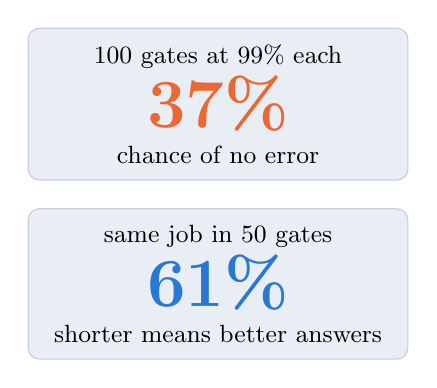
\begin{tikzpicture}
  \node[card,text width=4.4cm] (a) {100 gates at 99\% each\\[0.2em]{\Huge\bfseries\color{iorange}37\%}\\[0.2em]chance of no error};
  \node[card,text width=4.4cm,below=0.35cm of a] {same job in 50 gates\\[0.2em]{\Huge\bfseries\color{iaccent}61\%}\\[0.2em]shorter means better answers};
\end{tikzpicture}
\end{column}
\end{columns}
\src{This product of gate fidelities is the ESP (estimated success probability), the score we report on hardware.}
\end{frame}
\note{A quantum program is a circuit, a list of gates. Hardware makes a small error on every gate, two-qubit gates are the
worst. The chance of no error is roughly the product of all gate fidelities, called ESP. An optimiser rewrites the
circuit into a shorter one that does exactly the same thing. If asked why not just better hardware: both help, and
optimisation is free at run time.}

% ================================================================ 3 the original method
\begin{frame}{The original method: swap a piece for a shorter one}
\centering
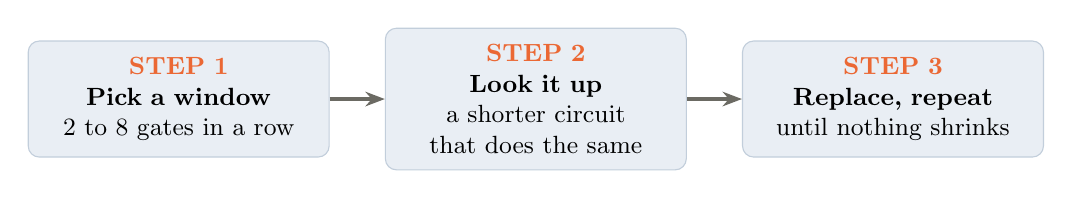
\begin{tikzpicture}[node distance=0.7cm]
  \node[card,text width=3.4cm] (s1) {\textcolor{iorange}{\textbf{STEP 1}}\\ \textbf{Pick a window}\\ 2 to 8 gates in a row};
  \node[card,text width=3.4cm,right=of s1] (s2) {\textcolor{iorange}{\textbf{STEP 2}}\\ \textbf{Look it up}\\ a shorter circuit that does the same};
  \node[card,text width=3.4cm,right=of s2] (s3) {\textcolor{iorange}{\textbf{STEP 3}}\\ \textbf{Replace, repeat}\\ until nothing shrinks};
  \draw[arr] (s1) -- (s2); \draw[arr] (s2) -- (s3);
\end{tikzpicture}
\vspace{1.2em}

\begin{columns}[c]
\begin{column}{0.26\textwidth}
\centering
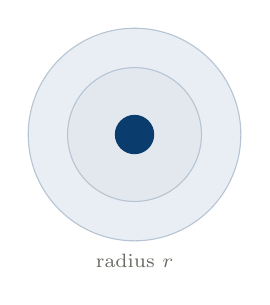
\begin{tikzpicture}
  \fill[ifoot] (0,0) circle (1.35); \draw[ibar!30] (0,0) circle (1.35);
  \fill[ibar!12] (0,0) circle (0.85); \draw[ibar!30] (0,0) circle (0.85);
  \fill[ibar] (0,0) circle (0.25);
  \node[font=\scriptsize,muted] at (0,-1.6) {radius $r$};
\end{tikzpicture}
\end{column}
\begin{column}{0.70\textwidth}
\textbf{The lookup table is a map of short circuits.}\\[0.3em]
\small Start from ``do nothing'' (the dot) and add one gate at a time. Every circuit reachable in at most $r$ steps is
stored with its shortest form. This map is the \textbf{compute graph}, and $r$ is the \textbf{database radius}.
The original paper uses $r=5$ or $6$.
\end{column}
\end{columns}
\src{Rosenhahn, Osborne and Hirche, New J.\ Phys.\ 27, 104509 (2025). Variants V1 (random search), V2 (database), V3 (database with a random forest).}
\end{frame}
\note{The paper we build on. Look at a short piece, find an equal but shorter piece in a precomputed table, swap, repeat.
The table comes from a compute graph: nodes are circuits (as matrices), edges add one gate, and the database holds
everything within radius r of the identity. Two knobs, window length w and radius r, explain everything later. If asked
why only 2 to 8 gates: the table grows exponentially with r.}

% ================================================================ 4 the two questions
{\setbeamercolor{background canvas}{bg=ibar}
\begin{frame}[plain]
\vspace{1.5em}
{\small\bfseries\color{iorange!70!white} TWO QUESTIONS THE ORIGINAL PAPER LEAVES OPEN}\\[1.6em]
\begin{columns}[T]
\begin{column}{0.46\textwidth}
{\fontsize{40}{40}\selectfont\bfseries\color{iorange!80!white}1}\\[0.6em]
{\Large\bfseries\color{white} How far from the best possible is it?}\\[0.8em]
{\color{white!75!ibar} They only compare with Qiskit, so a 45-gate result cannot be judged. Is the best 40 gates, or 10?}
\end{column}
\begin{column}{0.46\textwidth}
{\fontsize{40}{40}\selectfont\bfseries\color{iaccent!60!white}2}\\[0.6em]
{\Large\bfseries\color{white} Does it help on circuits people actually run?}\\[0.8em]
{\color{white!75!ibar} Their tests use random circuits, a few fixed gates, every qubit linked to every other, and only count gates.}
\end{column}
\end{columns}
\end{frame}}
\note{The whole motivation. Question 1 needs ground truth, the true shortest length, which nobody had. Question 2 needs
real algorithm circuits on realistic devices with real error rates and limited connectivity, against strong compilers.}

% ================================================================ 5 ground truth
\begin{frame}{Question 1: we computed the true shortest circuit}
\begin{columns}[c]
\begin{column}{0.38\textwidth}
\small
Their gates on 3 qubits only make a finite set of operations. We listed \textbf{all 92,897,280} of them and stored the
exact shortest length of each.\\[0.8em]
So for any test circuit we know the \opt{\textbf{best possible answer}}, not just ``better than Qiskit''.\\[0.8em]
Beyond this set (Clifford+T gates) we do the same for 2 qubits, and hide a known short core inside long circuits.
\end{column}
\begin{column}{0.60\textwidth}
\centering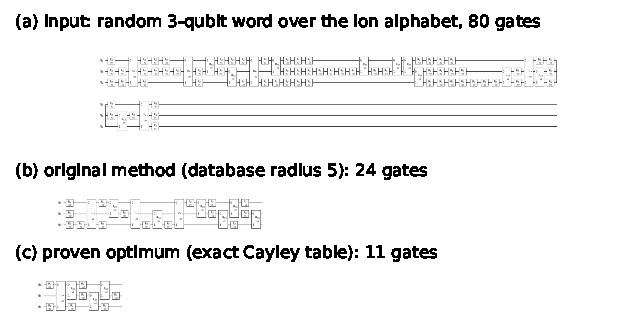
\includegraphics[width=\linewidth]{figs/fig_example_paper.pdf}
\end{column}
\end{columns}
\src{Example: an 80-gate random circuit. The original method stops at 24 gates. The proven optimum is 11.}
\end{frame}
\note{The gates in the original paper are plus or minus 90 degree rotations, which only generate the Clifford group. On 3
qubits it is finite, so we enumerated it, 92.9 million elements, with the exact distance of each from the identity. That
is ground truth. If asked whether this is a Clifford trick: the optimiser we test never uses this table, it is only the
referee. For non-Clifford gates we computed exact 2-qubit Clifford+T distances and planted benchmarks.}

% ================================================================ 6 why it falls short
\begin{frame}{Why it falls short: the lookup table is too small}
\begin{columns}[c]
\begin{column}{0.56\textwidth}
\centering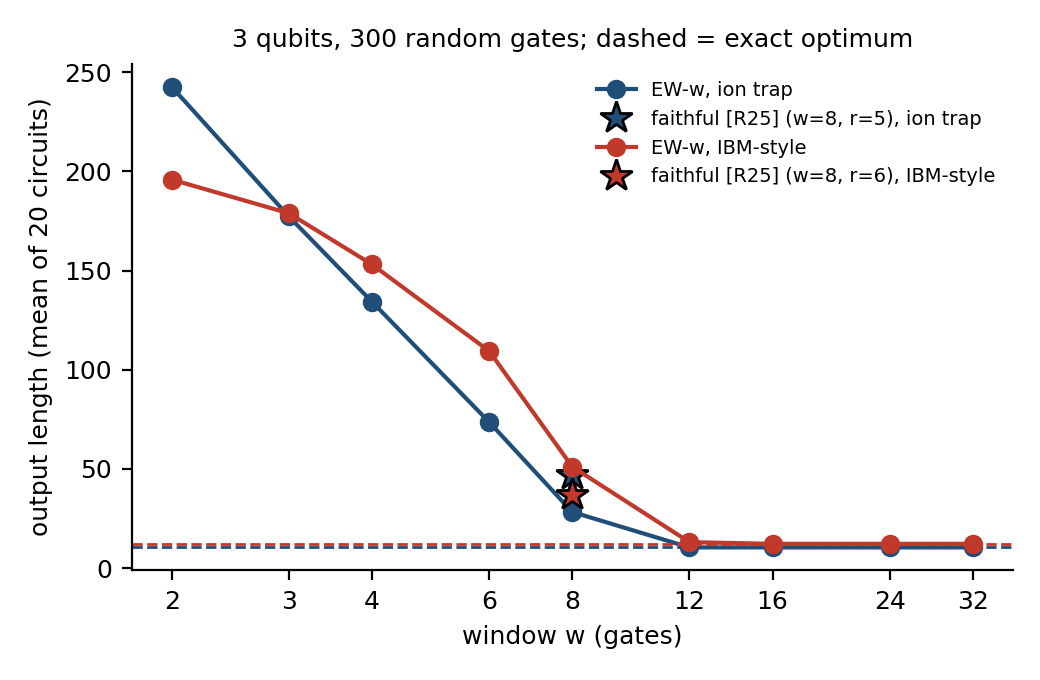
\includegraphics[width=\linewidth]{figs/ext_window.png}
\end{column}
\begin{column}{0.42\textwidth}
\small Two knobs decide the result. Both must be large enough.\\[0.8em]
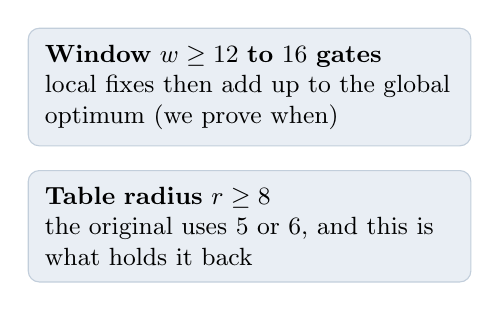
\begin{tikzpicture}
  \node[card,text width=5.2cm,align=left] (w) {\textbf{Window $w \ge 12$ to $16$ gates}\\ local fixes then add up to the global optimum (we prove when)};
  \node[card,text width=5.2cm,align=left,below=0.3cm of w] {\textbf{Table radius $r \ge 8$}\\ the original uses 5 or 6, and this is what holds it back};
\end{tikzpicture}
\end{column}
\end{columns}
\src{3 qubits, 300 random gates, 20 circuits. Stars: the original method. Dashed: the proven optimum.}
\end{frame}
\note{With ground truth we can explain the gap. Once the window reaches 12 (ion) or 16 (IBM-style) gates a simple sweep hits
the proven optimum on all 20 circuits. The stars are the original method at window 8. At window 8, raising r from 5 to
unlimited cuts the excess from 46 to 18 gates, and with w at least 12 and r at least 8 the excess is at most 2 gates. Our
theorem predicts both conditions. If asked about cost: a bigger table is a one-time precomputation, stored as hashed keys.}

% ================================================================ 7 results on their tests
\begin{frame}{On their own tests, we land on the optimum}
\centering\small
\begin{tabular}{l r r r r}
\toprule
Test (mean gates, 300 in) & Qiskit & Original & Ours & Best possible\\
\midrule
3 qubits, ion gates        & 127 & \orig{47.1} & \ours{10.8} & \opt{10.4}\\
3 qubits, IBM-style gates  & 104 & \orig{36.8} & \ours{12.5} & \opt{12.2}\\
4 qubits, ion gates        & 165 & \orig{78.8} & \ours{46.1} & \opt{at least 11}\\
4 qubits, IBM-style gates  & 141 & \orig{76.0} & \ours{51.4} & \opt{at least 13}\\
15 qubits (500 in)         & 332 & \orig{336}  & \ours{328}  & \opt{unknown}\\
\bottomrule
\end{tabular}
\vspace{1em}

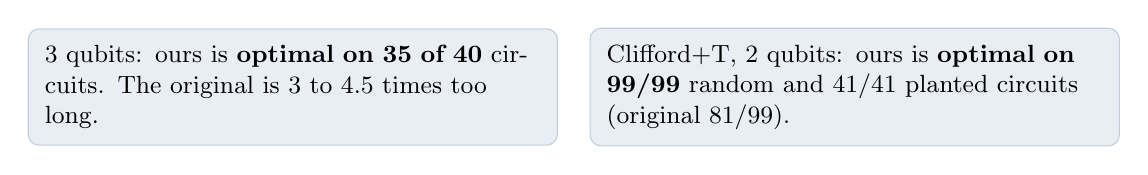
\begin{tikzpicture}
  \node[card,text width=6.3cm,align=left] (a) {3 qubits: ours is \textbf{optimal on 35 of 40} circuits. The original is 3 to 4.5 times too long.};
  \node[card,text width=6.3cm,align=left,right=0.4cm of a] {Clifford+T, 2 qubits: ours is \textbf{optimal on 99/99} random and 41/41 planted circuits (original 81/99).};
\end{tikzpicture}
\end{frame}
\note{On the 3-qubit tests our general optimiser is within 0.4 gates of the proven optimum and optimal on 35 of 40. At 4
qubits the optimum is too big to compute, but we prove a lower bound, so the remaining gap is at most about 4 times. At 15
qubits on random circuits everything, Qiskit included, lands within 4 percent, because random circuits leave little local
structure, which we also prove. If asked: ours does not use the Clifford table.}

% ================================================================ 8 our optimiser
\begin{frame}{Question 2: our optimiser, built for real devices}
\centering
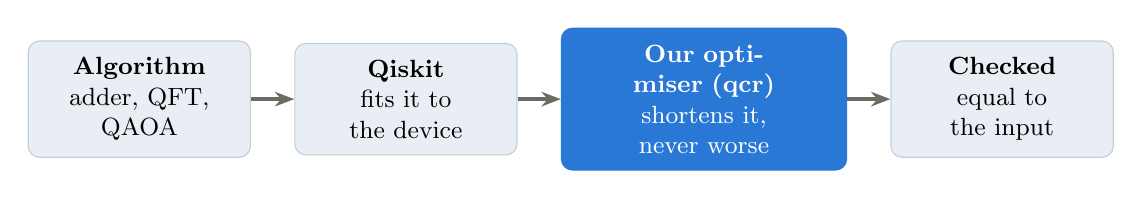
\begin{tikzpicture}[node distance=0.55cm]
  \node[card,text width=2.4cm] (a) {\textbf{Algorithm}\\ adder, QFT, QAOA};
  \node[card,text width=2.4cm,right=of a] (b) {\textbf{Qiskit}\\ fits it to the device};
  \node[hot,text width=3.2cm,right=of b] (c) {\textbf{Our optimiser (qcr)}\\ shortens it, never worse};
  \node[card,text width=2.4cm,right=of c] (d) {\textbf{Checked}\\ equal to the input};
  \draw[arr] (a) -- (b); \draw[arr] (b) -- (c); \draw[arr] (c) -- (d);
\end{tikzpicture}
\vspace{1.2em}

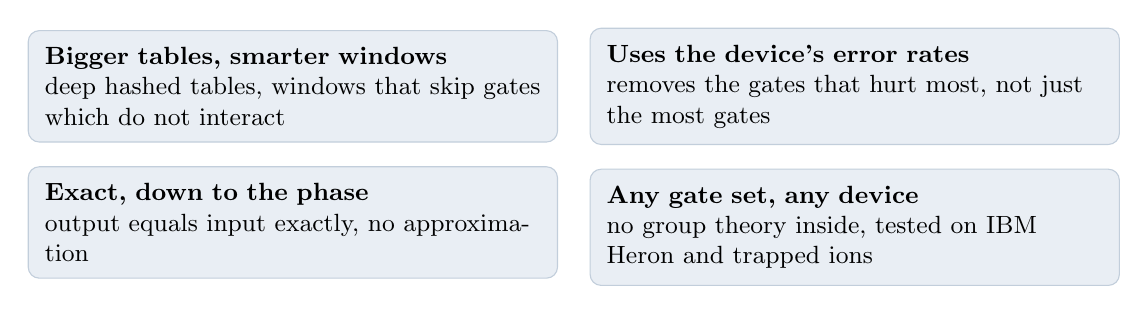
\begin{tikzpicture}
  \node[card,text width=6.3cm,align=left] (p) {\textbf{Bigger tables, smarter windows}\\ deep hashed tables, windows that skip gates which do not interact};
  \node[card,text width=6.3cm,align=left,right=0.4cm of p] (q) {\textbf{Uses the device's error rates}\\ removes the gates that hurt most, not just the most gates};
  \node[card,text width=6.3cm,align=left,below=0.3cm of p] (r) {\textbf{Exact, down to the phase}\\ output equals input exactly, no approximation};
  \node[card,text width=6.3cm,align=left,below=0.3cm of q] {\textbf{Any gate set, any device}\\ no group theory inside, tested on IBM Heron and trapped ions};
\end{tikzpicture}
\end{frame}
\note{Same simple idea, local swaps from a table, with what we found fixed. Tables are deeper and hashed. Windows are
convex, reaching past gates on other qubits that commute out of the way. The cost uses calibrated error rates. Outputs are
exactly equal including global phase. It runs after Qiskit, so any compiler can use it. Approximate and state-aware modes
exist and are in the paper, the headline numbers are exact mode.}

% ================================================================ 9 hardware suite
\begin{frame}{60 real algorithm circuits on IBM Heron}
\begin{columns}[T]
\begin{column}{0.60\textwidth}
\small
\begin{tabular}{l r r r}
\toprule
Compared with Qiskit level 3 & 2-qubit & all gates & ESP\\
\midrule
Qiskit level 3            & 1.00 & 1.00 & 1.00\\
TKET                      & 1.02 & 1.71 & 1.16\\
\ours{Ours, after level 3} & \ours{0.98} & \ours{0.87} & \ours{1.03}\\
\ours{Ours, after level 1} & \ours{1.00} & \ours{0.84} & \ours{1.21}\\
BQSKit level 3 (approx.)  & 0.85 & 1.20 & 1.22\\
\ours{Ours, after BQSKit}  & \ours{0.85} & \ours{1.01} & \ours{1.25}\\
\bottomrule
\end{tabular}
\end{column}
\begin{column}{0.38\textwidth}
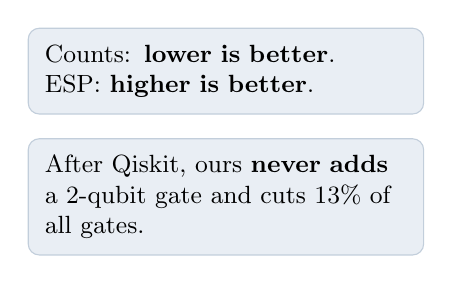
\begin{tikzpicture}
  \node[card,text width=4.6cm,align=left] (a) {Counts: \textbf{lower is better}.\\ ESP: \textbf{higher is better}.};
  \node[card,text width=4.6cm,align=left,below=0.3cm of a] {After Qiskit, ours \textbf{never adds} a 2-qubit gate and cuts 13\% of all gates.};
\end{tikzpicture}
\end{column}
\end{columns}
\takeaway{BQSKit finds better 2-qubit structure but leaves many 1-qubit gates. Run ours after it and you get both:
its 2-qubit savings and 16\% fewer gates, still exact.}
\src{58 circuits compared, 2 to 12 qubits. Trapped-ion results point the same way, with smaller margins.}
\end{frame}
\note{The suite: Nam arithmetic, QASMBench, QFT, QAOA, Trotter steps and more, for IBM Heron and a trapped-ion model,
relative to Qiskit level 3. Ours after level 3 never adds a two-qubit gate and removes 13 percent of all gates. BQSKit
is strongest on two-qubit gates because it resynthesises blocks numerically, but its outputs are approximate and full of
single-qubit rotations. Ours after BQSKit keeps its savings and removes 16 percent more gates, exactly. Also in the
paper: real error rates as the cost lower noisy-simulation TVD from 0.137 to 0.088 on Heron, and noise-aware layout
matters even more, about 1.6 times in ESP. If asked why ESP from level 1 is higher here: partly Qiskit's level 1 layout.}

% ================================================================ 10 large circuits
\begin{frame}{It scales: circuits of 14 to 100 qubits}
\centering
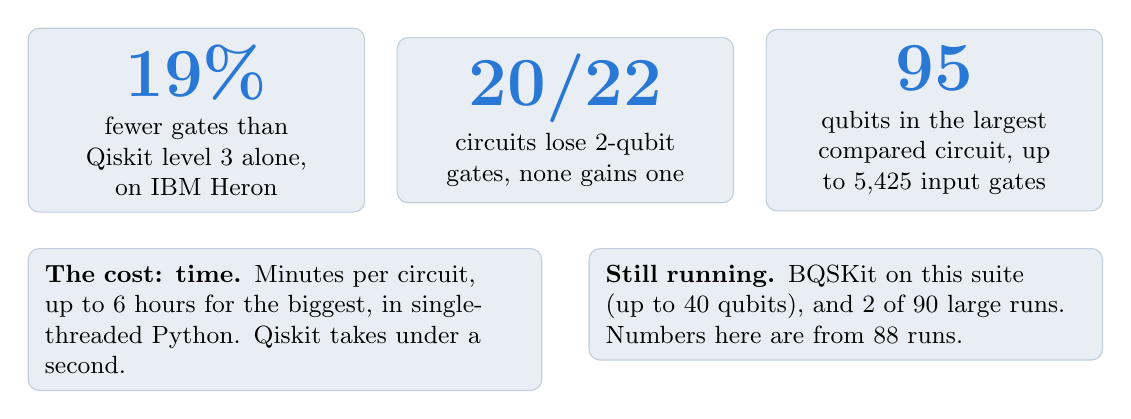
\begin{tikzpicture}[node distance=0.4cm]
  \node[card,text width=3.85cm] (a) {{\Huge\bfseries\color{iaccent}19\%}\\[0.3em] fewer gates than Qiskit level 3 alone, on IBM Heron};
  \node[card,text width=3.85cm,right=of a] (b) {{\Huge\bfseries\color{iaccent}20/22}\\[0.3em] circuits lose 2-qubit gates, none gains one};
  \node[card,text width=3.85cm,right=of b] (c) {{\Huge\bfseries\color{iaccent}95}\\[0.3em] qubits in the largest compared circuit, up to 5,425 input gates};
  \node[card,text width=6.1cm,align=left,below=0.45cm of a.south west,anchor=north west] (d) {\textbf{The cost: time.} Minutes per circuit, up to 6 hours for the biggest, in single-threaded Python. Qiskit takes under a second.};
  \node[card,text width=6.1cm,align=left,anchor=north east] at (d.north -| c.east) {\textbf{Still running.} BQSKit on this suite (up to 40 qubits), and 2 of 90 large runs. Numbers here are from 88 runs.};
\end{tikzpicture}
\src{45 Nam/VOQC circuits. Product-formula circuits excluded, as Qiskit drops their tiny rotations approximately.}
\end{frame}
\note{The 45 larger Nam/VOQC circuits, 14 to 100 qubits, on the 133-qubit Heron model and an all-to-all ion model. After
Qiskit level 3 on Heron we remove 19 percent of all gates and about 2 percent of two-qubit gates, on 20 of 22 comparable
circuits, never adding one. ESP goes up 1.12 times on the circuits where ESP is meaningful. On ions Qiskit already does
well and we mostly match it. The cost is run time. If asked about ESP from level 1: at this scale it is lower than level 3,
because Qiskit's level 3 layout matters more than the gates we remove. If asked about pf circuits: Qiskit level 3 removes
their 1e-7 rad rotations approximately, so the comparison would not be like for like.}

% ================================================================ 11 correctness
\begin{frame}{How we know every output is correct}
\centering
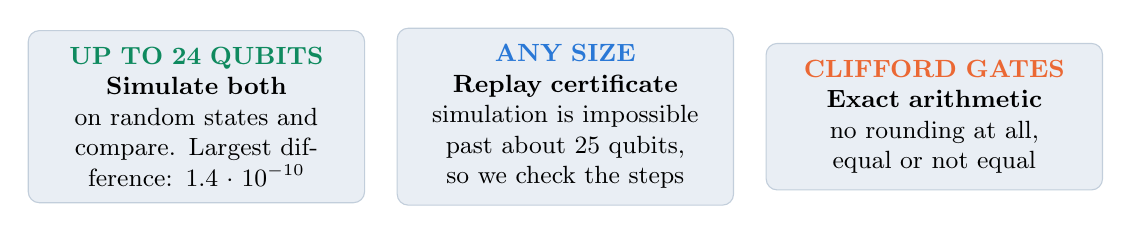
\begin{tikzpicture}[node distance=0.4cm]
  \node[card,text width=3.85cm] (a) {\textcolor{igreen}{\textbf{UP TO 24 QUBITS}}\\ \textbf{Simulate both}\\ on random states and compare. Largest difference: $1.4\cdot10^{-10}$};
  \node[card,text width=3.85cm,right=of a] (b) {\textcolor{iaccent}{\textbf{ANY SIZE}}\\ \textbf{Replay certificate}\\ simulation is impossible past about 25 qubits, so we check the steps};
  \node[card,text width=3.85cm,right=of b] (c) {\textcolor{iorange}{\textbf{CLIFFORD GATES}}\\ \textbf{Exact arithmetic}\\ no rounding at all, equal or not equal};
\end{tikzpicture}
\vspace{1em}

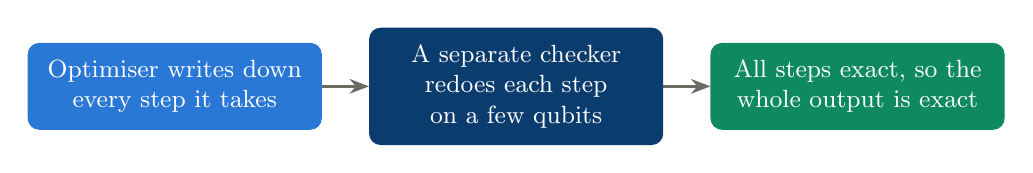
\begin{tikzpicture}[node distance=0.6cm]
  \node[hot,text width=3.3cm] (x) {Optimiser writes down every step it takes};
  \node[card,fill=ibar,draw=ibar,text=white,text width=3.3cm,right=of x] (y) {A separate checker redoes each step on a few qubits};
  \node[card,fill=igreen,draw=igreen,text=white,text width=3.3cm,right=of y] (z) {All steps exact, so the whole output is exact};
  \draw[arr] (x) -- (y); \draw[arr] (y) -- (z);
\end{tikzpicture}
\takeaway{Large suite: 171 of 176 outputs certified, each check under 7 seconds. The other 5 hit an old checker limit and are being re-run.}
\end{frame}
\note{Three layers. Up to 24 qubits we simulate input and output on random states. Beyond that simulation is out of reach,
and MQT QCEC gave no answer on routed 23-qubit adders. So the optimiser logs every step and an independent checker
replays them. Each step touches a few qubits, so cost grows with the number of steps, not the width, and it shares no code
or tables with the optimiser. Clifford and Clifford+T use exact arithmetic. If asked about the 5 pending: the first
checker checked the final phase fix as one block, which can span more than 12 qubits. The fixed checker does it piece by
piece, and the re-runs so far passed.}

% ================================================================ 12 what is left
\begin{frame}{What is left before submission}
\centering\small
\begin{tabular}{l l}
\toprule
Item & Status\\
\midrule
BQSKit on the large suite, 5 certificate re-checks & running\\
Fairer ESP reporting for very large circuits       & done\\
More baselines (VOQC, Quartz, QUESO)               & next\\
Several random seeds, with error bars              & next\\
Ablation: which part of the optimiser matters      & next\\
Runs on real IBM hardware                          & last, needs access\\
\bottomrule
\end{tabular}
\takeaway{In one line: the original method is 3 to 4.5 times off the optimum, we can prove it, and a general exact
optimiser closes that gap and still helps on real circuits up to 95 qubits.}
\end{frame}
\note{Be upfront about limits, it heads off most questions. BQSKit at scale and the re-checks are running. ESP at 50 or more
qubits is around 1e-10, so we now average only where ESP is meaningful and also give the median. Reviewers will want more
baselines, several seeds and an ablation, so those come next. Real hardware comes last because it needs IBM access and
queue time. Everything reported so far is verified, and the code and raw results will be public.}

\end{document}
